\documentclass{report}
\usepackage{graphicx, tikz-cd, float, titlepic, booktabs} % Required for inserting images
\usepackage{pgfplots}
\usepackage{multicol}
\usepackage{makecell}
\pgfplotsset{compat=1.15}
\usepackage{mathrsfs}
\usetikzlibrary{arrows}
\usepackage{amsmath, amssymb, amsthm, amsfonts, siunitx, physics, gensymb}
\AtBeginDocument{\RenewCommandCopy\qty\SI}
\usepackage[version=4]{mhchem}
\usepackage[most,many,breakable]{tcolorbox}
\usepackage{xcolor, fancyhdr, varwidth}
\usepackage[Glenn]{fncychap}
%Options: Sonny, Lenny, Glenn, Conny, Rejne, Bjarne, Bjornstrup
\usepackage{hyperref, cleveref}
\usepackage{icomma, enumitem} %comma as decimal and continue enumerate with [resume]
\usepackage{plimsoll} %use standard state symbol with \stst
\usepackage[danish]{babel}
\renewcommand{\cellalign}{cl}
\renewcommand{\theadalign}{cl}
\renewcommand\theadfont{\bfseries}
%%%%%%%%%%%%%%%%%%%%%%%%%%%%%%
% SELF MADE COLORS
%%%%%%%%%%%%%%%%%%%%%%%%%%%%%%
\definecolor{myg}{RGB}{56, 140, 70}
\definecolor{myb}{RGB}{45, 111, 177}
\definecolor{myr}{RGB}{199, 68, 64}
\definecolor{mytheorembg}{HTML}{F2F2F9}
\definecolor{mytheoremfr}{HTML}{00007B}
\definecolor{mylenmabg}{HTML}{FFFAF8}
\definecolor{mylenmafr}{HTML}{983b0f}
\definecolor{mypropbg}{HTML}{f2fbfc}
\definecolor{mypropfr}{HTML}{191971}
\definecolor{myexamplebg}{HTML}{F2FBF8}
\definecolor{myexamplefr}{HTML}{88D6D1}
\definecolor{myexampleti}{HTML}{2A7F7F}
\definecolor{mydefinitbg}{HTML}{E5E5FF}
\definecolor{mydefinitfr}{HTML}{3F3FA3}
\definecolor{notesgreen}{RGB}{0,162,0}
\definecolor{myp}{RGB}{197, 92, 212}
\definecolor{mygr}{HTML}{2C3338}
\definecolor{myred}{RGB}{127,0,0}
\definecolor{myyellow}{RGB}{169,121,69}
\definecolor{myexercisebg}{HTML}{F2FBF8}
\definecolor{myexercisefg}{HTML}{88D6D1}
%%%%%%%%%%%%%%%%%%%%%%%%%%%%%%%%%%%%%%%%%%%%%%%%%%%%%%%%%%%%%%%%%%%%%%
% Box environments for theorems and problems
%%%%%%%%%%%%%%%%%%%%%%%%%%%%%%%%%%%%%%%%%%%%%%%%%%%%%%%%%%%%%%%%%%%%%
\setlength{\parindent}{1cm}
%================================
% Question BOX
%================================
\newtcbtheorem[]{question}{Opgave}{enhanced,
	before skip=2mm,after skip=2mm, colback=red!5,colframe=red!80!black,boxrule=0.5mm,
	attach boxed title to top left={xshift=1cm,yshift*=1mm-\tcboxedtitleheight}, varwidth boxed title*=-3cm,
	boxed title style={frame code={
					\path[fill=tcbcolback]
					([yshift=-1mm,xshift=-1mm]frame.north west)
					arc[start angle=0,end angle=180,radius=1mm]
					([yshift=-1mm,xshift=1mm]frame.north east)
					arc[start angle=180,end angle=0,radius=1mm];
					\path[left color=tcbcolback!60!black!65!red,right color=tcbcolback!60!black!65!red,
						middle color=tcbcolback!80!black!65!red!1!red]
					([xshift=-2mm]frame.north west) -- ([xshift=2mm]frame.north east)
					[rounded corners=1mm]-- ([xshift=1mm,yshift=-1mm]frame.north east)
					-- (frame.south east) -- (frame.south west)
					-- ([xshift=-1mm,yshift=-1mm]frame.north west)
					[sharp corners]-- cycle;
				},interior engine=empty,
		},
	fonttitle=\bfseries,
	title={#2},#1}{def}


\makeatletter
\newtcbtheorem{Question}{Opgave}{enhanced,
	breakable,
	colback=white,
	colframe=myb!80!black,
	attach boxed title to top left={yshift*=-\tcboxedtitleheight},
	fonttitle=\bfseries,
	title={#2},
	boxed title size=title,
	boxed title style={%
			sharp corners,
			rounded corners=northwest,
			colback=tcbcolframe,
			boxrule=0pt,
		},
	underlay boxed title={%
			\path[fill=tcbcolframe] (title.south west)--(title.south east)
			to[out=0, in=180] ([xshift=5mm]title.east)--
			(title.center-|frame.east)
			[rounded corners=\kvtcb@arc] |-
			(frame.north) -| cycle;
		},
	#1
}{def}
\makeatother
%================================
% DEFINITION BOX
%================================

\newtheorem{defin}{Definition}[section] % Creates a new counter, number within section

\newtcbtheorem[number within=section, use counter*=defin]{Definition}{Definition}{enhanced,
	before skip=2mm,after skip=2mm, colback=red!5,colframe=red!80!black,boxrule=0.5mm,
	attach boxed title to top left={xshift=1cm,yshift*=1mm-\tcboxedtitleheight}, varwidth boxed title*=-3cm,
	boxed title style={frame code={
					\path[fill=tcbcolback]
					([yshift=-1mm,xshift=-1mm]frame.north west)
					arc[start angle=0,end angle=180,radius=1mm]
					([yshift=-1mm,xshift=1mm]frame.north east)
					arc[start angle=180,end angle=0,radius=1mm];
					\path[left color=tcbcolback!60!black,right color=tcbcolback!60!black,
						middle color=tcbcolback!80!black]
					([xshift=-2mm]frame.north west) -- ([xshift=2mm]frame.north east)
					[rounded corners=1mm]-- ([xshift=1mm,yshift=-1mm]frame.north east)
					-- (frame.south east) -- (frame.south west)
					-- ([xshift=-1mm,yshift=-1mm]frame.north west)
					[sharp corners]-- cycle;
				},interior engine=empty,
		},
	fonttitle=\bfseries,
	title={#2},#1}{def}

\newtcbtheorem[number within=section]{definition}{Definition}
{%
	enhanced,
	breakable,
	colback = red!5,
	frame hidden,
	boxrule = 0sp,
	borderline west = {2pt}{0pt}{solid, red!75!black},
	sharp corners,
	detach title,
	before upper = \tcbtitle\par\smallskip,
	coltitle = red!75!black,
	fonttitle = \bfseries\sffamily,
	description font = \mdseries,
	separator sign none,
	segmentation style={solid, red!75!black},
}
{th}

\newtcbtheorem{theo}%
    {Theorem}{}{theorem}
\newtcolorbox{prob}[1]{colback=red!5!white,colframe=red!50!black,fonttitle=\bfseries,title={#1}}

%================================
% NOTE BOX
%================================

\usetikzlibrary{arrows,calc,shadows.blur}
\tcbuselibrary{skins}
\newtcolorbox{note}[1][]{%
	enhanced jigsaw,
	colback=gray!20!white,%
	colframe=gray!80!black,
	size=small,
	boxrule=1pt,
	title=\textbf{Note:},
	halign title=flush center,
	coltitle=black,
	breakable,
	drop shadow=black!50!white,
	attach boxed title to top left={xshift=1cm,yshift=-\tcboxedtitleheight/2,yshifttext=-\tcboxedtitleheight/2},
	minipage boxed title=1.5cm,
	boxed title style={%
			colback=white,
			size=fbox,
			boxrule=1pt,
			boxsep=2pt,
			underlay={%
					\coordinate (dotA) at ($(interior.west) + (-0.5pt,0)$);
					\coordinate (dotB) at ($(interior.east) + (0.5pt,0)$);
					\begin{scope}
						\clip (interior.north west) rectangle ([xshift=3ex]interior.east);
						\filldraw [white, blur shadow={shadow opacity=60, shadow yshift=-.75ex}, rounded corners=2pt] (interior.north west) rectangle (interior.south east);
					\end{scope}
					\begin{scope}[gray!80!black]
						\fill (dotA) circle (2pt);
						\fill (dotB) circle (2pt);
					\end{scope}
				},
		},
	#1,
}
%================================
% EXAMPLE BOX
%================================
\newtcbtheorem[number within=section, use counter from=definition]{Example}{Example}
{%
	colback = myexamplebg
	,breakable
	,colframe = myexamplefr
	,coltitle = myexampleti
	,boxrule = 1pt
	,sharp corners
	,detach title
	,before upper=\tcbtitle\par\smallskip
	,fonttitle = \bfseries
	,description font = \mdseries
	,separator sign none
	,description delimiters parenthesis
}
{ex}
%================================
% THEOREM BOX
%================================

\tcbuselibrary{theorems,skins,hooks}
\newtcbtheorem[number within=section, use counter from=definition]{Theorem}{Theorem}
{%
	enhanced,
	breakable,
	colback = mytheorembg,
	frame hidden,
	boxrule = 0sp,
	borderline west = {2pt}{0pt}{mytheoremfr},
	sharp corners,
	detach title,
	before upper = \tcbtitle\par\smallskip,
	coltitle = mytheoremfr,
	fonttitle = \bfseries\sffamily,
	description font = \mdseries,
	separator sign none,
	segmentation style={solid, mytheoremfr},
}
{th}

%%%%%%%%%%%%%%%%%%%%%%%%%%%%%%%%%%%%%%%%%%%%%%%%%%%%%%%%%%%%%%%%%
% SELF MADE COMMANDS
%%%%%%%%%%%%%%%%%%%%%%%%%%%%%%
\newcommand{\sol}{\setlength{\parindent}{0cm}\textbf{\textit{Løsning:}}\setlength{\parindent}{1cm}}
%%%%%%%%%%%%%%%%%%%%%%%%%%%%%%%%%
\usepackage[tmargin=2cm,rmargin=1in,lmargin=1in,margin=0.85in,bmargin=2cm,footskip=.2in]{geometry}\pagestyle{fancy}
\lhead{Minrui Kevin Zhou 3.b}
\rhead{Opgavesæt 9}

\title{Opgavesæt 9\\
{\Large \textbf{3.b kemi A}}}
\author{Kevin Zhou}
\date{\today}

\begin{document}
\maketitle
\begin{note}
  Databog fysik kemi (2007) er benyttet ved beregningerne.
\end{note}
\section*{Opgave 1: Adipinsyre}
\sol \\
\textbf{a.}
Siden de to carboxylsyregrupper er de funktionelle grupper med højst prioritering, skal navnet ende på -disyre.
Derudover indeholder den længste kæde af C-atomer netop seks C-atomer, og hexan må da være i navnet (se \cref{fig:adipinsyre}).
Da der kun er én mulighed for, hvor de to syregrupper kan sidde, så behøver vi ikke angive nummeret på C-atomerne, hvorpå de sidder.
Det systematiske navn for adipinsyre bliver således hexandisyre.
\begin{figure}[H]
\begin{center}
  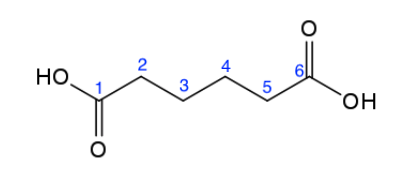
\includegraphics[width=0.8\textwidth]{adipinsyre.png}
\end{center}
\caption{Navngivning af adipinsyre}
\label{fig:adipinsyre}
\end{figure}

\textbf{b.}
Lad \ce{H2Adp} betegne adipinsyre.
Så må titreringsreaktionen fra start til første ækvivalenspunkt (bemærk, at adipinsyre er dihydron) så være
\begin{equation*}
\begin{split}
  \ce{H2Adp(aq) + OH-(aq) -> HAdp-(aq) + H2O(l)}.
\end{split}
\end{equation*}
Det ses, at reaktionsforholdet mellem \ce{NaOH} og adipinsyre er 1:1.
\begin{figure}[H]
\begin{center}
  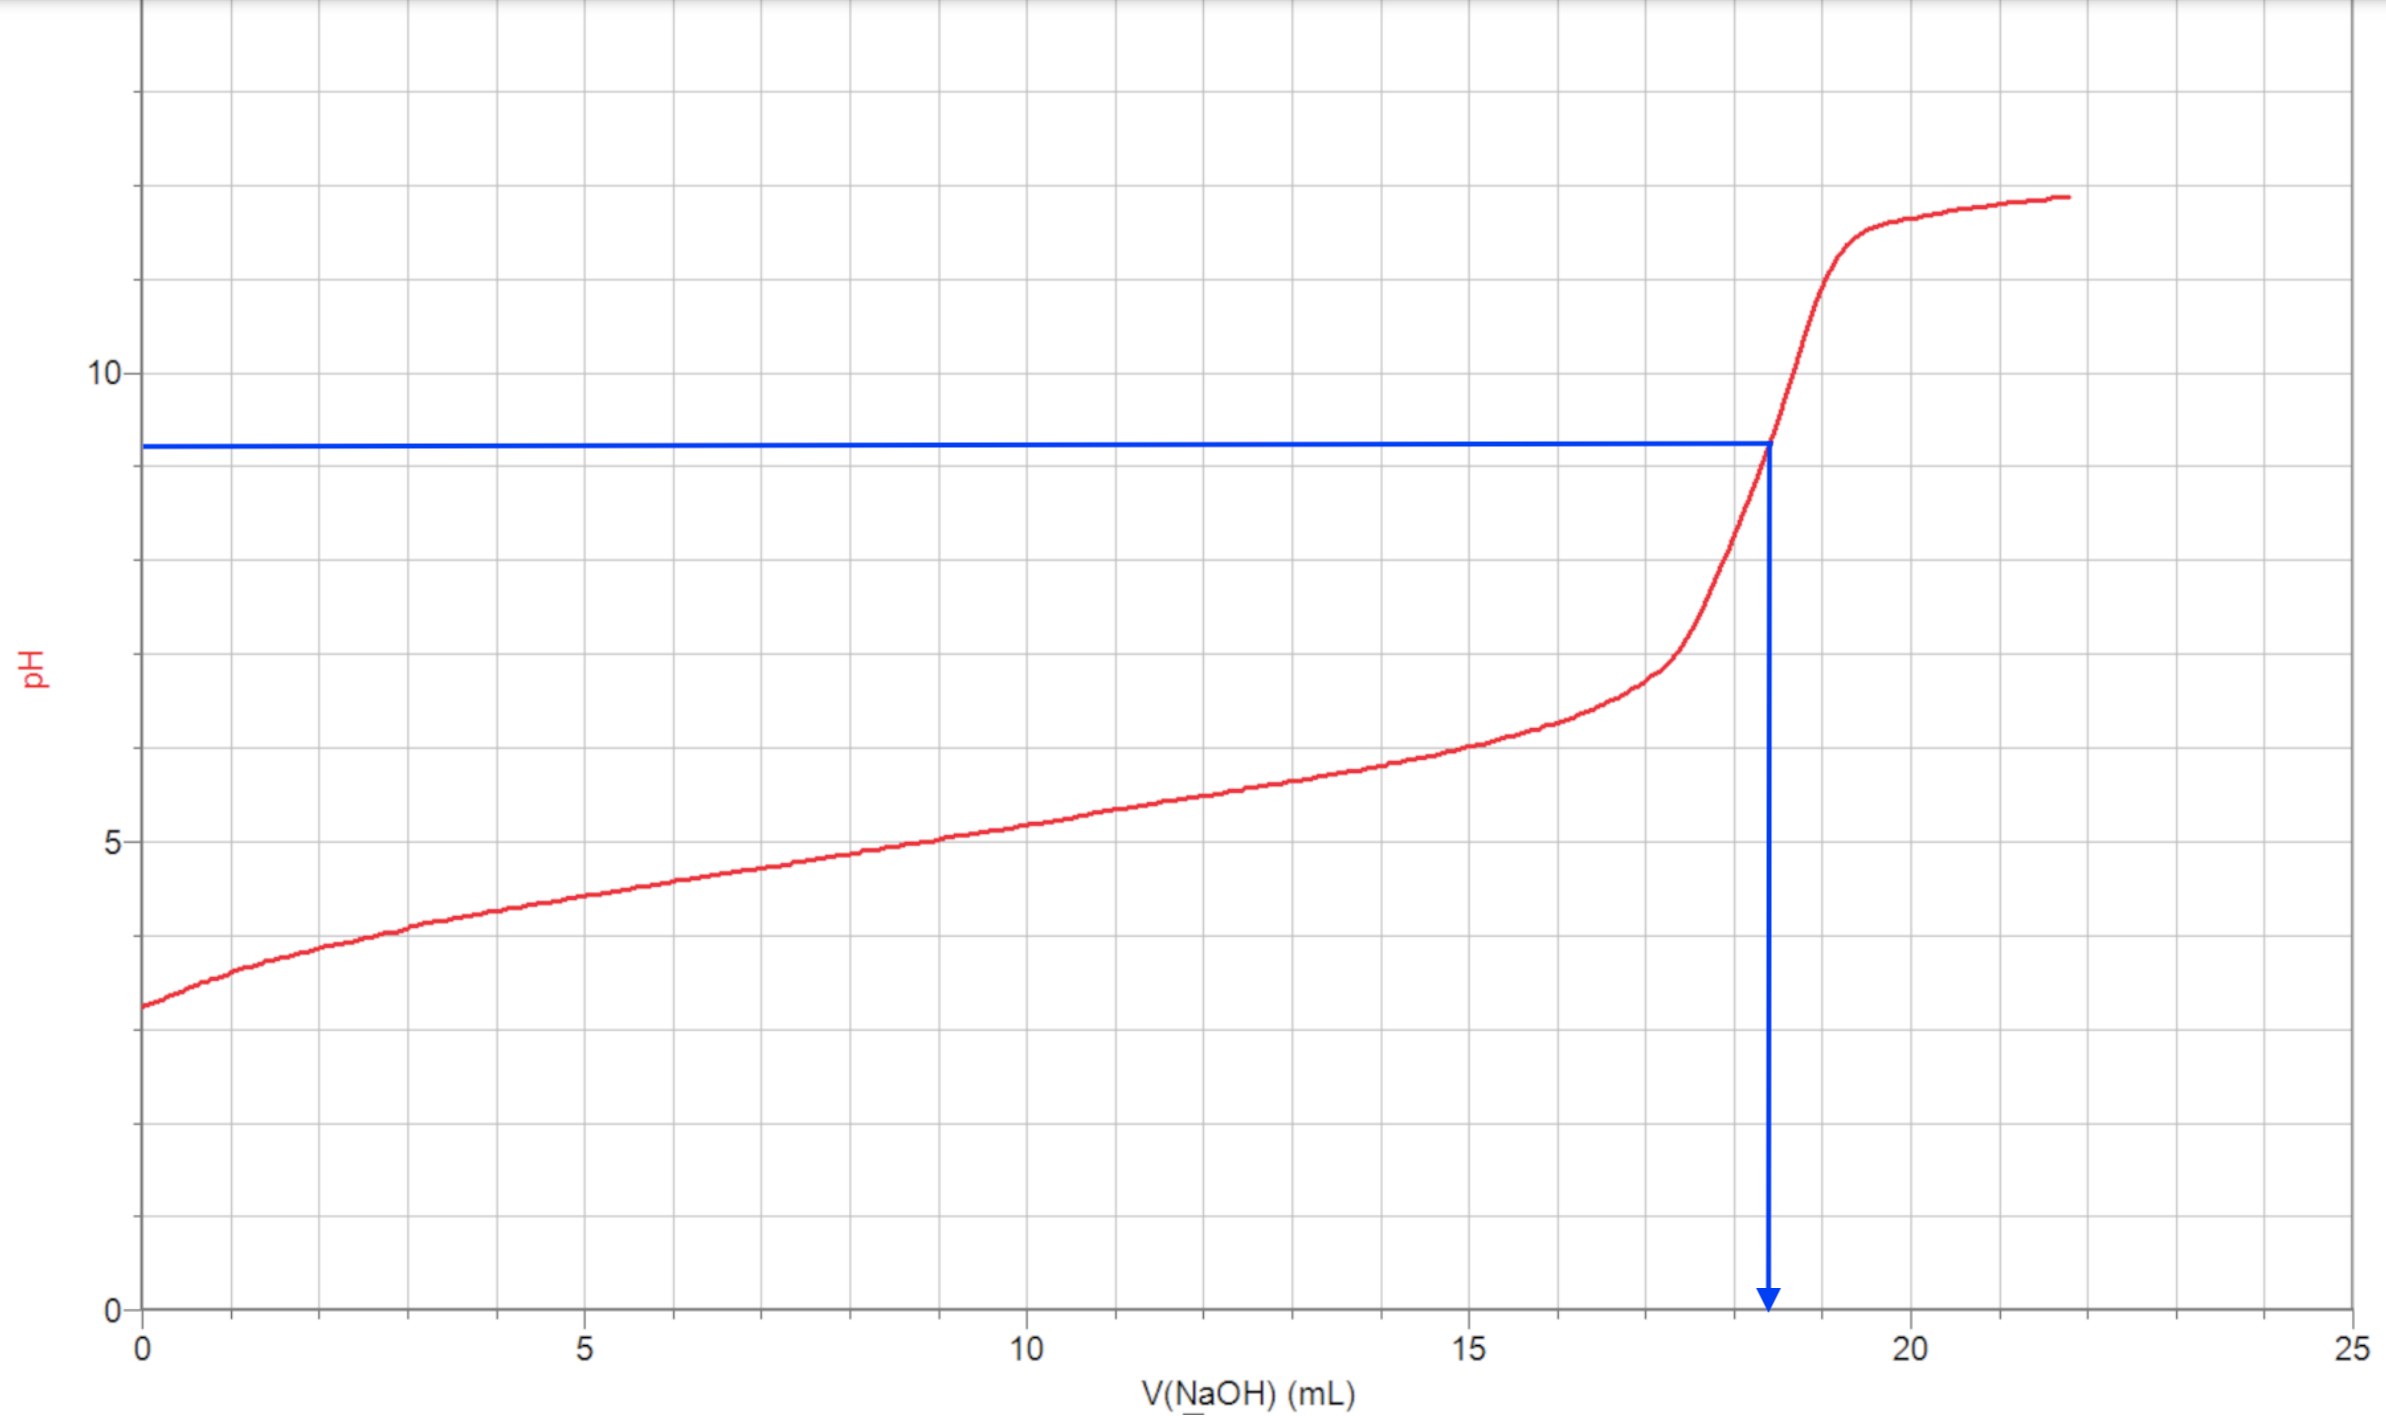
\includegraphics[width=0.65\textwidth]{titrer.png}
\end{center}
\caption{Aflæsning på titrerkurven}
\label{fig:titrer}
\end{figure}
Ved det første ækvivalenspunkt må der gælde, at $n(\ce{H2Adp})=n(\ce{NaOH} )$, hvor $n(\ce{H2Adp} )$ er stofmængden af adipinsyre i den oprindelige mættede opløsning. 
Vi aflæser på titrerkurven (se \cref{fig:titrer}), at det tilsatte volumen \ce{NaOH}-opløsning ved første ækvivalenspunkt er $V(\ce{NaOH} )= 18,4 \;\unit{mL}$.
Da vi fra videoen har, at stofmængdekoncentrationen af \ce{NaOH}-opløsningen er $c(\ce{NaOH} )=0,0891 \;\unit{\textsc{m}} $ og volumen af den mættede opløsning er $V(\text{adipinsyre})=5,00 \;\unit{mL}$, så kan vi udregne $c(\ce{H2Adp})$.
\begin{equation*}
\begin{split}
  c(\ce{H2Adp})&=\frac{n(\ce{H2Adp} )}{V(\ce{H2Adp})}\\
  &=\frac{c(\ce{NaOH}) \cdot V(\ce{NaOH})}{V(\ce{H2Adp} )}\\
  &=\frac{0,0891 \;\unit{\textsc{m}} \cdot 18,4 \;\unit{mL} }{5,00 \;\unit{mL} }\\
  &\approx 0,328 \;\unit{\textsc{m}}
\end{split}
\end{equation*}
Stofmængdekoncentrationen af adipinsyre i den mættede opløsning er altså $c(\ce{H2Adp})=0,329 \;\unit{\textsc{m}} $.\\[1ex]
\textbf{c.}
For at bestemme molekylformlen for esteren, finder vi først den empiriske formel.
Fra elementaranalysen har vi, at der i 100 g af stoffet må være
\begin{equation*}
\begin{split}
  n(\ce{C} )&=\frac{65,09 \;\unit{g} }{12,01 \;\unit{g/mol} }= 5,4197 \;\unit{mol} \\
  n(\ce{H} )&=\frac{10,14 \;\unit{g} }{1,008 \;\unit{g/mol} }= 10,0595 \;\unit{mol} \\
  n(\ce{O})&=\frac{24,77 \;\unit{g} }{16,00 \;\unit{g/mol} }= 1,5481 \;\unit{mol} 
\end{split}
\end{equation*}
Vi beregner nu stofmængdeforholdene.
\begin{equation*}
\begin{split}
  \frac{n(\ce{C} )}{n(\ce{O} )}&=\frac{5,4197 \;\unit{mol} }{1,5481 \;\unit{mol} }= 3,5008 \approx 3,5 \\
  \frac{n(\ce{H} )}{n(\ce{O} )}&=\frac{10,0595 \;\unit{mol} }{1,5481 \;\unit{mol} }=6,4979 \approx 6,5
\end{split}
\end{equation*}
Forholdet mellem stofmængderne af C, H og O er altså med stor nøjagtighed 7:13:2.
Esterens empiriske formel må da være \ce{C7H13O2}.
Imidlertid har vi fra esterens strukturformel (se \cref{fig:esterstruk}), at esteren netop indeholder fire O-atomer (for R betegner alkylgrupper).
Vi ganger da den empiriske formel op med 2, og får, at molekylformlen for esteren må være \ce{C14H26O4}.
\begin{figure}[H]
\begin{center}
  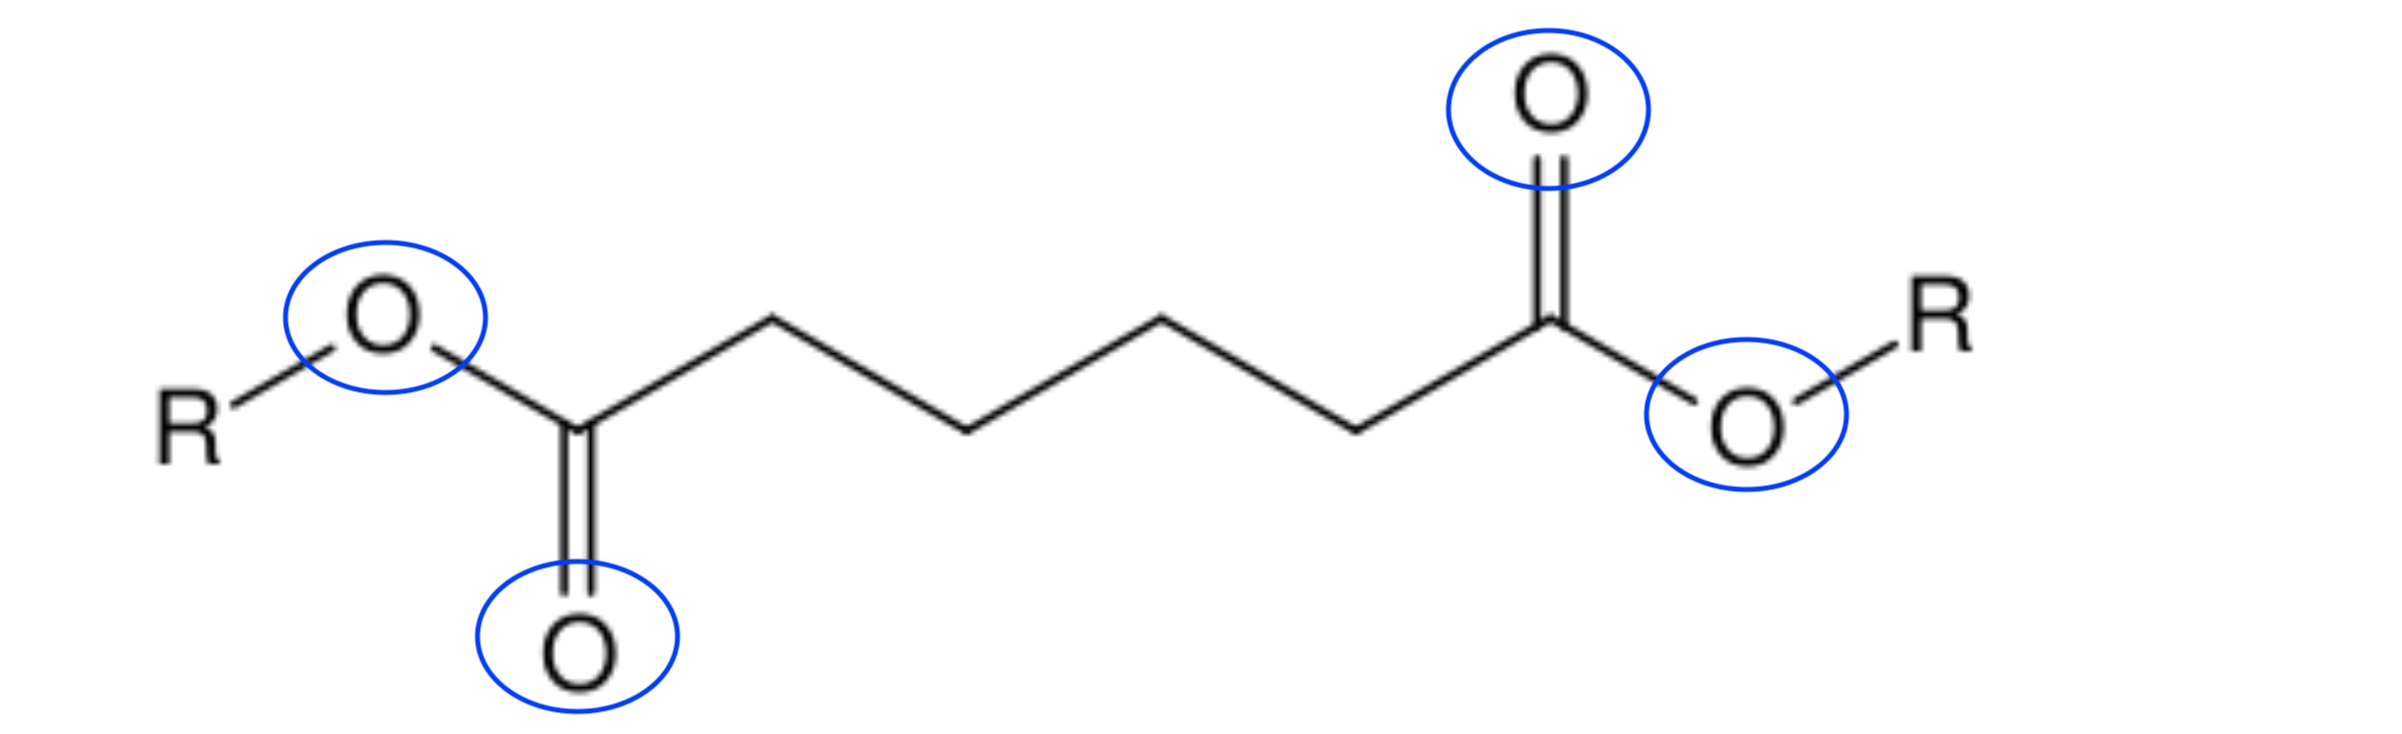
\includegraphics[width=0.7\textwidth]{esterstruk.png}
\end{center}
\caption{Esteren indeholder netop fire O-atomer}
\label{fig:esterstruk}
\end{figure}
\noindent \textbf{d.}
Vi betragter \ce{^1H}-NMR-spektret for alkoholen.
En opsummerende tabel ses i tabel \ref{tab:HNMR}.

\begin{table}[H]
\centering
\begin{tabular}{@{}lllllll@{}}
\toprule
  \makecell{Signal\\nr.} & \makecell{Kemisk skift\\(aflæst)\\$\delta$/ppm}& \makecell{Integral/areal\\(relativt antal ækvi-\\valente \ce{^1H}-atomer)}  & Opsplitning & \makecell{Antal nabo-\\\ce{^1H}'er}  & Tilordning & \makecell{Kemisk skift\\(tabel)\\$\delta$/ppm} \\
\midrule
  1 & 0,93 & 3 & Triplet & 2 & \ce{C\textbf{H}3-CH2} & 0,9\\
  2 & 1,39 & 2 & Sekstet & 5 & \ce{-CH2-C\textbf{H}2-CH3} & 1,3\\
  3 & 1,53 & 2 & Kvintet & 4 & \ce{-CH2-C\textbf{H}2-CH2-OH} & 1,5 \\
  4 & 2,24 & 1 & Singlet & 0 & \ce{-OH} & 0,5-5 \\
  5 & 3,62 & 2 & Triplet & 2 & \ce{-CH2-C\textbf{H}2-OH} & 3,5 \\
\bottomrule
\end{tabular}
\caption{Tilordning af absorptionsbånd i \ce{^1H}-NMR-spektret}
\label{tab:HNMR}
\end{table}

Der er fem signaler i spektret, hvilket betyder, at der er fem forskellige grupper af ækvivalente \ce{^1H}-kerner.
Siden R er en alkylgruppe, så fremgår det klart fra arealerne af signal nr. 1, 2, 3 og 5, at alkoholen indeholder én \ce{CH3}-gruppe og tre \ce{CH2}-grupper.
Signal nr. 4 kan tilordnes \ce{OH}-gruppen.

Fra opsplitningerne har vi så, at \ce{^1H}-kernerne hørende til signal 1 må koble til de to \ce{^1H}-kerner hørende til signal 2.
Derudover fremgår det også fra opsplitningerne samt kemiske skift, at \ce{^1H}-kernerne hørende til signal nr. 5 må koble til \ce{^1H}-kernen hørende til hydroxy-gruppen i signal nr. 4 samt \ce{^1H}-kernerne hørende til signal nr. 3.
Til sidst må \ce{^1H}-kernerne hørende til signal 3 både koble til \ce{^1H}-kernerne hørende til signal nr. 5 og dem, der hører til signal nr. 2.

Altså vil det sige, at vi har \ce{CH3}-gruppen bundet til en \ce{CH2}-gruppe, der er bundet til en \ce{CH2}-gruppe, der er bundet til endnu en \ce{CH2}-gruppe, der er bundet til \ce{OH}-gruppen. 
Strukturformlen for alkoholen ses i \cref{fig:HNMRalk}, hvor \ce{^1H}-kernerne, der svarer til hvert signal er numereret.
\begin{figure}[H]
\begin{center}
  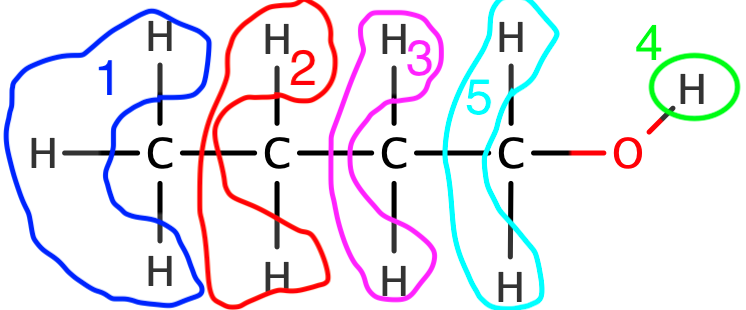
\includegraphics[width=0.8\textwidth]{HNMRalk.png}
\end{center}
\caption{Strukturen for \ce{R-OH} }
\label{fig:HNMRalk}
\end{figure}

\section*{Opgave 2:    Avobenzon - et kemisk filter i solcreme}
\sol \\
\textbf{a.}
Vi ser fra absorptionsspektret (\cref{fig:absorption}), at absorptionen er størst i området $330 \;\unit{nm} $ til $380 \;\unit{nm} $, hvilket ligger indenfor området af UV-A. 
Altså beskytter avobenzon især mod ultraviolet stråling fra solen i form af UV-A.
\begin{figure}[H]
\begin{center}
  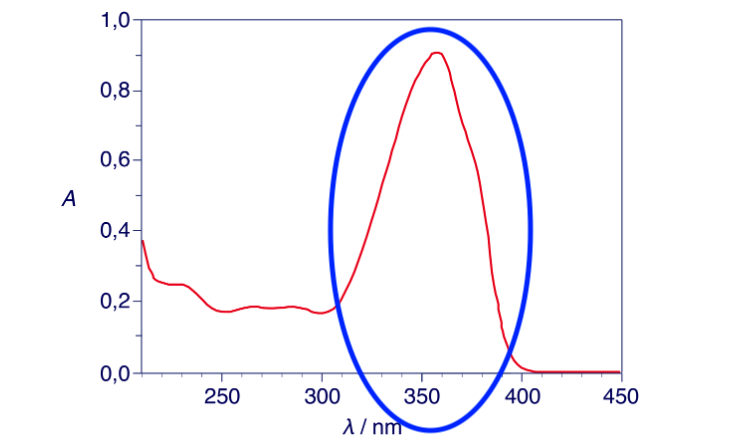
\includegraphics[width=0.8\textwidth]{absorption.png}
\end{center}
\caption{Absorptionsspektrum}
\label{fig:absorption}
\end{figure}
\noindent \textbf{b.}
Avobenzon B kan udvise stereoisomeri, da der ikke er omdrejningsfrihed ved dobbeltbindingen (se \cref{fig:stereo}), og der sidder fire distinkte grupper på de to C-atomer, hvorimellem dobbeltbindingen sidder.

Vi ser nu på prioriteringerne af substituenterne på C-atomerne, hvorimellem dobbeltbindingen sidder.
Grupperne med højst prioritet er markeret med 1 i \cref{fig:stereo}, og de laveste med 2.
Det ses, at grupperne med højst prioritet sidder på samme side af dobbeltbindingen, hvilket vil sige, at der er tale om Z-formen.

\begin{figure}[H]
\begin{center}
  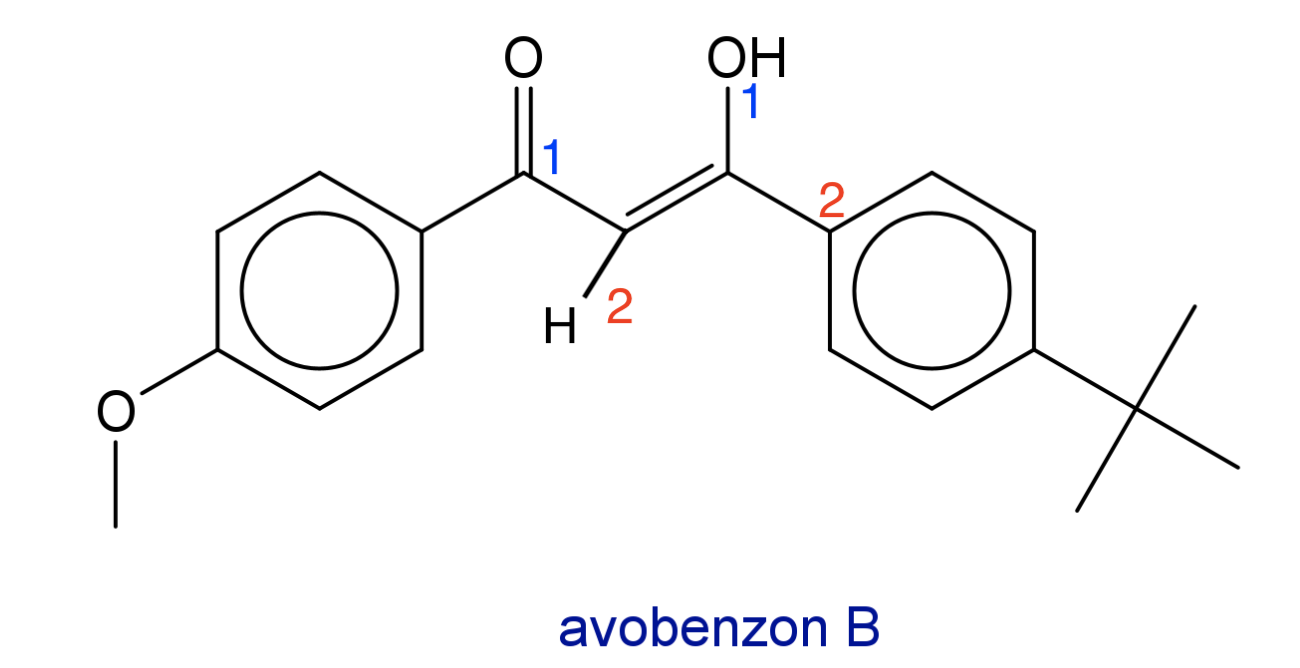
\includegraphics[width=0.8\textwidth]{stereo.png}
\end{center}
\caption{Avobenzon B kan udvise stereoisomeri}
\label{fig:stereo}
\end{figure}
\noindent \textbf{c.}



\end{document}
